\chapter{Physical Development of Donation System}\label{ch:C}
\section{Overview of the idea}
As the design system and implementation of the project went parallel, the changes from one to another were made accordingly. However only frontend part was similar to the design project that was stated at the beginning. 
\par
Main problem of the interaction is understanding between two opposite sides, it's a big work on developing user interface part, because in some cases there is no ability to show people the same web-site as it was established at the beginning. 'Donor project' website was done in the most simple way possible - HTML+CSS+JavaScript. In addition the usage of framework Jinja2 helped to avoid code repetition and code overlapping, so this technology was used fully in this project.
\par
Backend part in the process of the development wasn't affected as much as frontend. This is because the information coming had slightly changed. The simplicity of using Flask as a backend service allowed to develop lightweight system, that doesn't require much storage and memory space. In general, Python3 language was optimal solution for the project, because in future scaling we can easily perform on a big amount of data and users as well as we do on a small amount.
\par
Originally Django was chosen as a framework to implement backend. But as we began working with Django, we have figured out, that a lot of functions and methods that there are in the framework we basically don't need. Flask has been positioning itself as a microservice framework. This was the perfect solution.
\par
Most of the development time was spent on creating logically correct and functioning database. As a database structure has to be normalized, the process of adapting data that we had to a form of a relational database was long. This is because there was a lot of data retrieval, deleting and adding different columns. But as we have our minimum value product, now the structure is perfectly fits in current system.

\section{Database development and maintaining}
Developing database is a process of constant brainstorming. There are a lot of methods of showing relationship between entities, but for this project we didn't have a lot of entities to connect and the database is simple. So the optimal solution of visual representation was showing relationships between entities in a table form.
\par
This method allows to visualize main tables that are used more often than others \cite{adrianne}, so whilst rewriting it, we have managed to normalize database faster and easier.
(see Figure \ref{fig:relations})
\par
As a database storing from the developer side using PostgreSQL v.12 was perfect solution. It has more complicated functionality which allows to maintain data fast and without a lot of editing inputs and outputs. PostgreSQL tries to conform with the SQL standard where such conformance does not contradict traditional features or could lead to poor architectural decisions \cite{postgresql}. Our goal was to develop logic and a strong base for further development, because when database is strictly organized, then there is no problems in further development.

\begin{figure}[h]
    \centering
    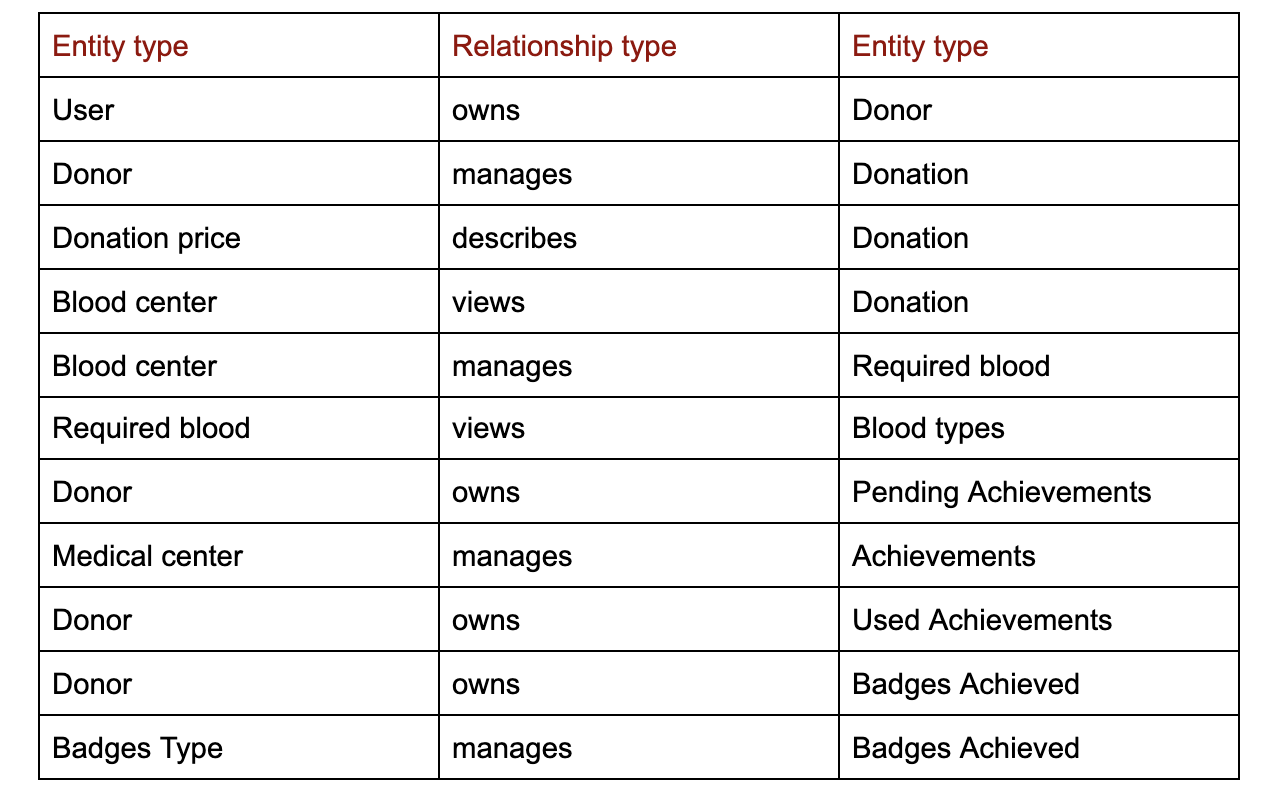
\includegraphics[scale=0.4]{figures/relations.png}
    \caption{Database table relations}
    \label{fig:relations}
\end{figure}

\section{Flask integration with PostgreSQL}
The connection between database and Flask doesn't require extra knowledge when both of the code structure and tables logic is organized. However there are some nuances that were used.
\par
\begin{lstlisting}

|-- Procfile
|-- app.py
|-- docker-compose.yml
|-- donorApp
|   |-- __init__.py
|   |-- donor.db
|   |-- helper_functions.py
|   |-- models.py
|   |-- routes.py
|   `-- templates

\end{lstlisting}

Flask application was structured in a different way, in order to simplify the view of each .py file. Main logic of all project configurations is stored in donorApp package. Basically everything that is related to database connection is stored as a configuration.

\begin{lstlisting}[language=Python]

app.config['SQLALCHEMY_DATABASE_URI'] =
'postgresql://<username>:<password>@localhost:<port>
/<database-name>'
app.config['SQLALCHEMY_TRACK_MODIFICATIONS'] = False
db = SQLAlchemy(app)

\end{lstlisting}
In order to manage the database the 'db' variable is used in main file of the project.
\par
Because SQLAlchemy is a common database abstraction layer and object relational mapper that requires a little bit of configuration effort, there is a Flask extension that handles that \cite{flasksql}.

\section{Docker-compose usage}
Quite often there are problems of implementing database packages on server-side. Also there might be difficulties in installing correct versions  and uninstalling unnecessary packages afterwards. So to avoid such consequences of running the project on broken database, docker-compose was chosen to maintain installation of the database package onto the server.
\par
The .yml file of the project is as simple as possible, because on this stage of the development we only use PostgreSQL. Docker calls the collection of files and instructions needed to run a software program an image \cite{docker}. 

\begin{lstlisting}[language=Python]

version: '3'
volumes:
  anketa_db_vol:

services:
  postgres:
    image: postgres:12
    volumes:
      - anketa_db_vol:/var/lib/postgresql/data
    environment:
      - POSTGRES_HOST=localhost
      - POSTGRES_PASSWORD=<password>
      - POSTGRES_DB=<database-name>
    ports:
      - "8432:5432"
    restart: always

\end{lstlisting}

\section{Backend implementation}
Architecture of Flask allowed fast and easy access to maintain, receive and publish data. The light structure demonstrates the code in the most simple way, so that even the developer who examines it for the first time will easily adapt to it. The example of the structure in the code snippet is a part of the project's method.

\begin{lstlisting}[language=Python]

@app.route('/logout', methods=['GET', 'POST'])
@login_required
def logout():
    logout_user()
    return redirect(url_for('main'))
    
\end{lstlisting}

\par
There is huge impact of the Flask database creation system. It allows to create entities without direct contact with database. This protects the structure and adds strict constraints in the development. So the ability to break tables or data stored is completely minimized.
\begin{lstlisting}[language=Python]
class User(db.Model, UserMixin):
    id = db.Column(db.Integer, primary_key=True)
    username = db.Column(db.String(80), unique=True)
    email = db.Column(db.String(120), unique=True)
    password = db.Column(db.String(120))
\end{lstlisting}
\par
It’s encouraged to use a package instead of a module for your flask application and drop the models into a separate module (Larger Applications) \cite{flasksql}.

\section{Frontend integration with Flask and Jinja2}
Jinja is a fast, expressive, extensible templating engine. Special placeholders in the template allow writing code similar to Python syntax \cite{jinja}.
Most common way to develop web-application on Python3 is to use this templating engine  to maintain frontend. 
\par
In 'Donor project' there are a lot of repeated blocks of code, which may be hard to follow, when the framework is not used. But when developing with Jinja2, it saves time and creates dynamic views, which don't require repeating. 
Also allowing to write code inside of the HTML code is huge advantage in frontend development. Whilst other frameworks like ReactJS require additional knowledge, Jinja offers common syntax that is perfect for small projects.
\begin{lstlisting}[language=HTML]





<!-- Preloader -->
<div id="page-loading-blocs-notifaction"></div>
<!-- Preloader END -->



\end{lstlisting}

Whilist developing front part there were a lot of changes from the original design that was made. This is justified by the functional requirements that were needed. 
\par
The interface of the web-design often doesn't have access to direct data that is being maintained from the user. In our case the development of the project started with the design idea and was followed by coding afterwards. Thus, we have common location of blocks, which doesn't break the original logic of wireframes, some of the design concept were not released in alpha-testing version.
\par
The concepts that haven't been used are following:
\begin{itemize}
  \item Main page detalized welcome image
  \item Representation of profile appointment scheduling
  \item The concept behind dropdown in header
\end{itemize}
\par
Though, those concept were not released, they were fully integrated into the system logically and have equivalent representation in 'Donor project' web-application.